\documentclass[11pt]{article}
\usepackage{mypackages}
\begin{document}

\maketitle

\subsection{Using deep learning for approximating functions}

In the last section we claimed that a neural network could be used to approximate the
state-value and action-value functions.
Generally for a function $f(x)$ the neural network tries to approximate $f^\sim(x)$
such that $f^\sim(x)$ varies the least from $f(x)$ for all $x$ in the input space\cite{DeepLearningBook}.
It does so by adjusting its parameters based on experience - data for which $f(x)$ is already known,
that can be used to compute how well the current approximation $f^\sim(x)$ is performing.

This data is exactly what is available in the agent-environtment model, when there is a natural terminal state,
since we can use the experienced actual returns to update the weights of the models.

\subsubsection{Layers, neurons and connections}

Instead of trying to approximate the function $f^\sim(x)$ directly,
a neural network uses a lot of less complex functions.
The beginning of the network can then be pretty simple, but by the combination of the results of
the simpler functions, it is able to solve complex problems in the end.
We call this structure a hierarchy of concepts, where each concept can be described in terms
of the previous and simpler concepts\cite{DeepLearningBook}.

More formally, a neural network consists of \textit{layers} that each represent a concept, which
when connected are able to solve the complex problem at hand.
With this definition of a neural network the approximation function $f^{\sim}(x)$ can be
defined as
\begin{equation}
    f^{\sim}(x) = f^{k}(f^{k-1}( \cdots f^{0}(x) \cdots))
\end{equation}
for a network with $k$ layers.
The only layers that have their dimensions restrained are the first and last, since they are defined by the
dimensions of the input data and the output of the true function, respectively.
This means the layers in between can have arbitrary shapes and
since we won't be seeing the output of those layers, we call them \textit{hidden layers}.
\begin{figure}[!h]
    \centering
    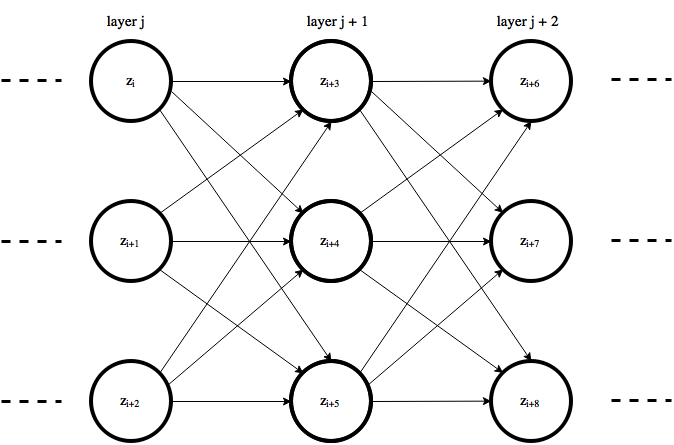
\includegraphics[width=10cm]{include/layers.png}
    \caption{A series of layers in a fully connected neural network.}
    \label{fig:layers}
\end{figure}
Each layer consists of a number of \textit{neurons} that are connected to the neurons of the
next layer.

Each neuron transforms its series of input signals into a single output signal which is sent to
each neuron in the following layer through \textit{weighted connections}, where
the weights of the connections define the importance of the signals.
The main purpose of hidden layers is to extract the key features of the original input
and they do so through the use of \textit{activation functions}.
Activation functions transform the weighted input signals into a single output that
describes a feature.
%%%% A drawing of a neuron “up close”
\begin{figure}[!h]
    \centering
    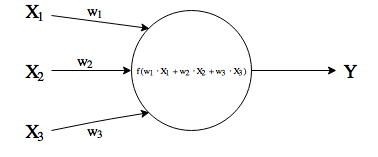
\includegraphics[width=10cm]{include/neuron.png}
    \caption{The structure of a single neuron with activation function $\alpha$.}
    \label{fig:neuron}
\end{figure}

The choice of activation function depends on the task the
network is supposed to solve.
E.g. when learning to play Atari games we generally want to estimate a policy.
This policy describes the probabilities of taking each available action
in the given state.
For this particular task the \textit{softmax} function can be used as activation function
in the output layer.
The softmax is defined as
\begin{equation}
    \text{softmax}(x) = \frac{exp(x_i)}{\sum\limits_{k=1}^K exp(x_k)}, \text{ for } i = 1, \dots, K
\end{equation}
for a $k$ dimensional input $x$ and is a generalization of the logistic function shown below.

\begin{figure}[!h]
    \centering
    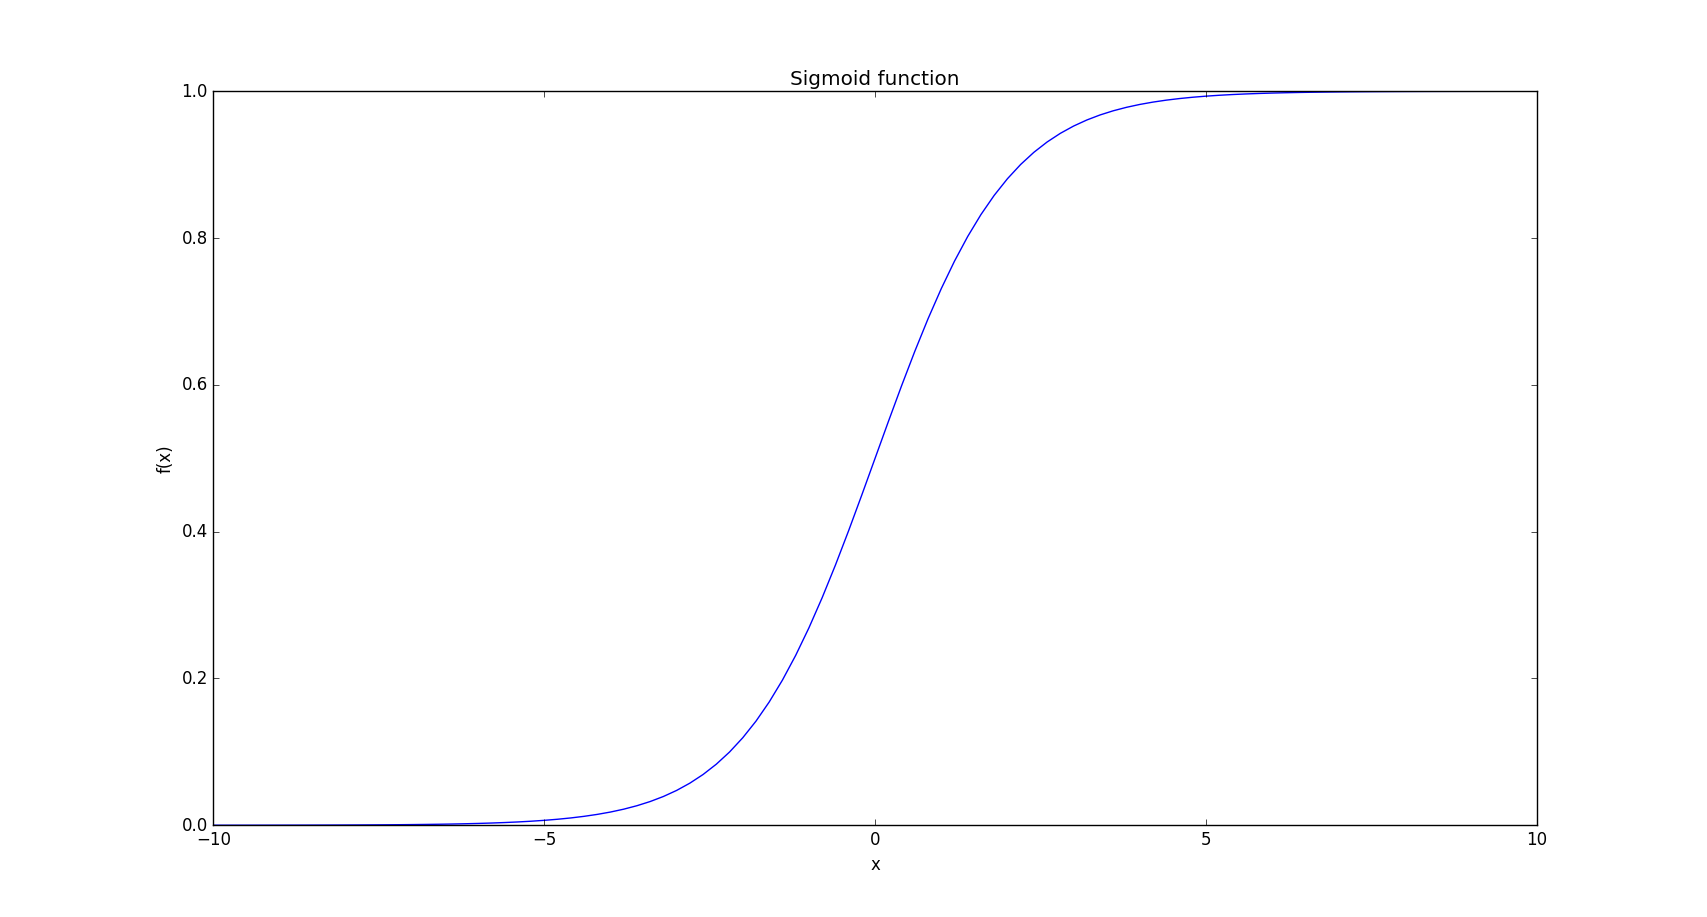
\includegraphics[width=15cm]{include/sigmoid.png}
    \caption{Plot of the logistic function.}
    \label{fig:softmax}
\end{figure}

Thus, the role of the output of each layer is to provide some additional
transformation from the features in order to complete the task the network
must perform\cite{DeepLearningBook}.

\subsubsection{Learning from multidimensional input}

To process the high dimensional frames from the Atari games we will be using
a \textit{convolutional neural network}.
A convolutional neural network typically performs three operations - a \textit{convolution},
a \textit{pooling} and an activation.

A convolution in two dimensions of a discrete image $I$ with filter kernel $K$
is given by 
\begin{equation}
    S(i, j) = (I \ast K)(i, j) = \sum\limits_m \sum\limits_n I(m, n) * K(i - m, j - n)
\end{equation}
where the kernel filter $K$ is a function $K : \R^{(d, k)} \to \R$.
A 2d convolutional layer uses the spatial structure in the input data to contruct a feature map
using the linear filter $K$.
Here the kernel filter is the weights of the connections in the network.
A non-linear function is then applied to the feature map elements resulting from the convolution,
and the process as a whole can be seen as neurons with shared weights\cite{IgelConv}.

In the network the kernel filter is used as weights and can be represented as a $d \times k$ dimensional matrix.
$$
K =
\begin{bmatrix}
    w_{1,1 } & w_{1, 2} & \hdots & w_{1, k} \\
    w_{2,1 } & w_{2, 2} & \hdots & w_{2, k} \\
    \vdots   &          & \ddots &          \\
    w_{d,1 } & w_{d, 2} & \hdots & w_{d, k} \\
\end{bmatrix}
$$
Each element in the resulting feature map is weighted based on its distance to the kernel center
and this can be seen as a neighbourhood function.

Given a $4 \times 4$ input image and a $3 \times 3$ kernel filter a convolution
would look like this
%%% 2d convolution
\begin{figure}[!h]\label{con2}
    \centering
    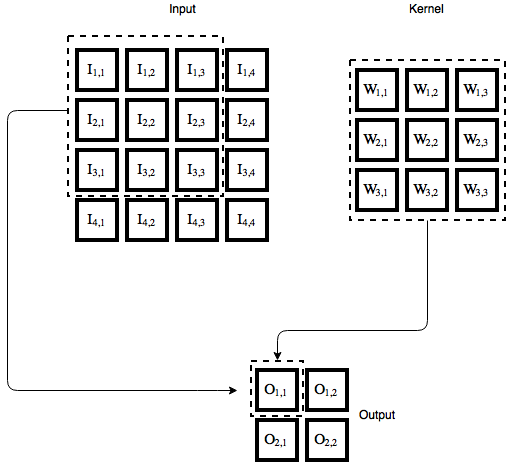
\includegraphics[width=10cm]{include/conv_2.png}
    \caption{A 2d convolution on an image which produces a \textit{feature} map.}
    \label{fig:conv}
\end{figure}

A problem with the raw convolution shown in figure \ref{conv2} is that
pixels at the boundary of the image are lost, which means some of the
features of the input may be lost.
To deal with this boundary issue we make use of zero padding.
We simply add zeros to the border of each image until the kernel
filter fits around each pixel.
This maintains the dimensions of the original image, since the pixels that are lost, now are
part of the padding.

%%% Zero padded 2d convolution
\begin{figure}[!h]\label{con2}
    \centering
    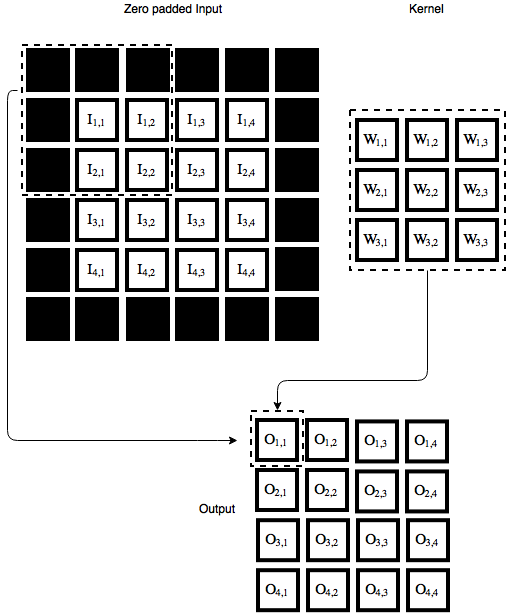
\includegraphics[width=10cm]{include/conv_2_zero_pad.png}
    \caption{The effect of zero padding the input image.}
    \label{fig:conv}
\end{figure}

Each pixel is now a weighted sum of its neighbouring pixels
which means that the result of the convolution is features from
the original input.
The feature map now consists of more separated objects than the original input,
which we means we can more safely reduce the dimensionality of without losing much information - 
this is called pooling and is used to support \textit{translation invariance}.
Translation invariance means that the features of the network should be able to
be extracted, regardless of their position in the feature map.
In an Atari game most objects move, while maintaining their original shape so being able to
extract information about objects independent of their position is very useful.

Instead of doing pooling and convolutions in two separate steps, we will be using 
convolutions \textit{with stride}.
What this means is that we we won't be be applying the convolution to 
every element of the input, but instead only the \textit{n'th} element.
An example of a one dimensional convolution with stride is visualized below.

%%%%% Strides
\begin{figure}[!h]\label{con2}
    \centering
    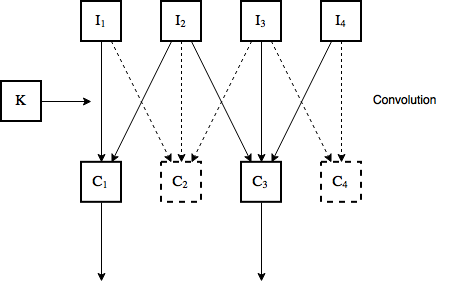
\includegraphics[width=10cm]{include/strides.png}
    \caption{A convolution with stride $2$ of an input using the kernel filter K. Only every second
        element of the resulting feature map is sent to the next layer.}
    \label{fig:conv}
\end{figure}

Here the convolution skips every second element, resulting in a downsampling
of the input.
The pooling operation usually computes the maximum or average of a region of a feature map,
and using convolution with strides emulates this behaviour since the convolution
can be seen as a weighted sum of neighbouring pixels.


%%% Move this to after Policy Gradients
%\subsubsection{Updating the weights of the network}

%A neural network is trained to minimize its total loss based on its \textit{loss
%function}.
%A loss function $\mathcal{L} : \R^K \to \R$ is supposed to describe how close the
%predictions are to the true result.
%In the reinforcement learning setting it is often difficult to estimate the
%true result.
%E.g. for a policy aproximator $\pi^{\sim}(A_t | S_t)$ we want to use the knowledge
%of wether or not action $A_t$ was  chosen in state $S_t$ to determine
%whether the probability of taking $A_t$ should be increased or decreased to
%reduce the loss of the network.
%Therefore the weights of the connections in the network are typically updated
%in a direction in the weight space.
%This direction describes how the weights should be updated to increases the
%probability of repeating the action $A_t$ the most on future visits to
%state $S_t$\cite{RLbook}.
%To find the direction we would use the \textit{gradient} of the probability of
%taking the action actually taken, since it exactly describes how to increate
%this probability.
%
%Now, this would increase the chance of picking action $A_t$ in state $S_t$ again,
%but we really only want to pick actions again that lead to a good return.
%Therefore the probability is generally updated proportionally to the
%return, since the network will then learn to favor actions that provide
%the highest return.
%
\end{document}
